
\begin{dang}{Bài toán quỹ tích và điểm cố định}
\end{dang}
\subsubsection{Ví dụ mẫu}
\begin{vd}
	Cho tứ diện $ABCD$ và $M$, $N$ là các điểm thay đổi trên các cạnh $AB$, $CD$ sao cho $\dfrac{AM}{MB}=\dfrac{CN}{ND}$.
	Chứng minh $MN$ luôn luôn song song với một mặt phẳng cố định.
	\loigiai{
		Do $\dfrac{AM}{MB}=\dfrac{CN}{ND}$ nên theo định lí Thales thì các đường thẳng $MN$, $AC$, $BD$ cùng song song với một mặt phẳng $(\beta)$. Gọi $(\alpha)$ là mặt phẳng đi qua $AC$ và song song với $BD$ thì $(\alpha)$ cố định và $(\alpha)\parallel(\beta)$ suy ra $MN$ luôn song song với $(\alpha)$ cố định.}
\end{vd}



\begin{vd}
	Cho tứ diện $ABCD$ và $M$, $N$ là các điểm thay đổi trên các cạnh $AB$, $CD$ sao cho $\dfrac{AM}{MB}=\dfrac{CN}{ND}$. Giả sử  $\dfrac{AM}{MB}=\dfrac{CN}{ND}=k>0$ và $P$ là một điểm trên cạnh $AC$ sao cho $PA=k PC$. Khi đó tìm thiết diện của hình chóp cắt bởi $(MNP)$.
	\loigiai{
		\begin{center}
			\begin{tikzpicture}[line join=round,line cap=round, font=\footnotesize, scale=1,>=stealth]
				\def\r{3}
				\path
				(0,0) coordinate (B)		
				(\r,0) coordinate (C)
				(-40:0.8*\r) coordinate (D)
				(75:1.1*\r) coordinate (A)
				($(B)!1.5!(C)$) coordinate (R)		
				($(B)!0.4!(D)$) coordinate (Q)
				($(C)!0.4!(D)$) coordinate (N)
				($(A)!0.4!(B)$) coordinate (M)
				($(A)!0.4!(C)$) coordinate (P)								
				;
				\draw (A)--(B)--(D)--(C)--(A)--(D)(M)--(Q)(N)--(P);		
				\draw[dashed](B)--(C)(P)--(M)(Q)--(N);		
				\foreach \x/\g in {A/160,B/180,C/60,D/-60,M/160,N/-60,P/60,Q/-100}\fill[black] (\x) circle (1pt)+(\g:.3)node{$\x$};
			\end{tikzpicture}
		\end{center}
		Ta có $\dfrac{AP}{PC}=k$, lúc này $MP\parallel BC$ nên $BC\parallel(MNP)$.\\
		Mặt khác,
		$\heva{&N\in(MNP)\cap(BCD)\\&BC\parallel(MNP)\\&BC\subset(BCD)}\Rightarrow(BCD)\cap(MNP)=NQ\parallel BC,\,Q\in BD$. \\
		Do đó thiết diện $MPNQ$ là hình thang.
	}
\end{vd}


\begin{vd}
	Cho tứ diện $ABCD$ và $M$, $N$ là các điểm thay đổi trên các cạnh $AB$, $CD$ sao cho  $\dfrac{AM}{MB}=\dfrac{CN}{ND}=k>0$ và $P$ là một điểm trên cạnh $AC$ sao cho $PA \neq k PC$. Tìm thiết diện của hình chóp cắt bởi $(MNP)$.
	\loigiai{
		Do $\dfrac{AP}{PC}\neq k$ nên trong $(ABC)$ gọi $R=BC\cap MP$.\\
		Trong $(BCD)$ gọi $Q=NR\cap BD$ thì thiết diện là tứ giác $MPNQ$.
	}
\end{vd}

\begin{vd}
	Cho tứ diện $ABCD$ và $M$, $N$ là các điểm thay đổi trên các cạnh $AB$, $CD$ sao cho  $\dfrac{AM}{MB}=\dfrac{CN}{ND}=k>0$ và $P$ là một điểm trên cạnh $AC$ sao cho $PA \neq k PC$. Tính theo $k$ tỉ số diện tích tam giác $MNP$ và diện tích thiết diện của hình chóp cắt bởi $(MNP)$.
	\loigiai{
		\begin{center}
			\begin{tikzpicture}[line join=round,line cap=round, font=\footnotesize, scale=1,>=stealth]
				\def\r{3}
				\path
				(0,0) coordinate (B)		
				(\r,0) coordinate (C)
				(-40:0.8*\r) coordinate (D)
				(75:1.1*\r) coordinate (A)
				($(B)!1.5!(C)$) coordinate (R)		
				($(B)!0.7!(D)$) coordinate (Q)
				($(A)!0.4!(B)$) coordinate (M)
				(intersection of C--D and R--Q) coordinate (N)
				(intersection of A--C and R--M) coordinate (P)
				(intersection of M--N and P--Q) coordinate (K)							
				;
				\draw (A)--(B)--(D)--(N)--(P)--(A)--(D)(P)--(R)--(N)(M)--(Q);		
				\draw[dashed](B)--(R)(P)--(C)--(N)--(M)--(P)--(Q)--(N);		
				\foreach \x/\g in {A/160,B/180,C/60,D/-60,M/160,N/-60,P/60,Q/-100,K/20,R/90}\fill[black] (\x) circle (1pt)+(\g:.3)node{$\x$};
			\end{tikzpicture}					
		\end{center}
		Gọi $K=MN\cap PQ$. Ta có $\dfrac{S_{MNP}}{S_{MPNQ}}=\dfrac{PK}{PQ}$.\\ 		
		Do $\dfrac{AM}{MB}=\dfrac{CN}{ND}$ nên theo định lí Thales đảo thì $AC$, $NM$, $BD$ lần lượt thuộc ba mặt phẳng song song với nhau và đường thẳng $PQ$ cắt ba mặt phẳng này tương ứng tại $P$, $K$, $Q$ nên áp dụng định lí Thales ta được $\dfrac{PK}{KQ}=\dfrac{AM}{MB}=\dfrac{CN}{ND}=k$\\
		$\Rightarrow\dfrac{PK}{PQ}=\dfrac{PK}{PK+KQ}=\dfrac{\dfrac{PK}{KQ}}{\dfrac{PK}{KQ}+1}=\dfrac{k}{k+1}$.	
	}
\end{vd}

\begin{vd}
	Cho hình chóp $S.ABCD$ có đáy $ABCD$ là hình bình hành tâm $O$ có $AC=a$, $BD=b$. Tam giác $SBD$ là tam giác đều. Một mặt phẳng $(\alpha)$ di động song song với mặt phẳng $(SBD)$ và đi qua điểm $I$ trên đoạn $AO$ và $AI=x$ ($0<x<a$). Tính diện tích thiết diện theo $a$, $b$ và $x$.
	\loigiai{
		\begin{center}
			
			\begin{tikzpicture}[line join=round,line cap=round, font=\footnotesize, scale=1,>=stealth]
				\def\r{3}
				\path
				(0,0) coordinate (A)		
				(\r,0) coordinate (B)
				(-130:0.6*\r) coordinate (D)			
				($(B)+(D)$) coordinate (C)
				($(A)!0.9!95:(B)$) coordinate (S)
				($(A)!0.5!(B)$) coordinate (M)
				($(A)!0.5!(D)$) coordinate (N)		
				($(S)!0.5!(A)$) coordinate (P)		
				($(A)!0.5!(C)$) coordinate (O)
				(intersection of A--C and M--N) coordinate (I)						
				;
				\draw (D)--(C)--(B)--(S)--(D)(C)--(S);
				\draw[dashed] (A)--(B)(S)--(A)(A)--(D)(N)--(M)--(P)--(N)(A)--(C)(B)--(D);	
				\foreach \x/\g in {S/160,A/60,B/0,C/-30,D/180,M/40,N/180,P/60,O/-90,I/-90}\fill[black] (\x) circle (1pt)+(\g:.3)node{$\x$};
			\end{tikzpicture}
		\end{center}
		Do	$I$ thuộc đoạn $OA$.\\
		Ta có $S_{SBD}=\dfrac{BD^2\sqrt{3}}{4}=\dfrac{b^2\sqrt{3}}{4}$, $\dfrac{S_{MNP}}{S_{SBD}}=\left(\dfrac{MN}{BD}\right)^2$.\\
		Do $MN\parallel BD\Rightarrow\dfrac{MN}{BD}=\dfrac{AI}{AO}=\dfrac{2x}{a}$\\
		$\Rightarrow S_{MNP}=\left(\dfrac{2x}{a}\right)^2S_{SBD}=\dfrac{b^2x^2\sqrt{3}}{a^2}$.
	}
\end{vd}

\subsubsection{Bài tập rèn luyện}
\Opensolutionfile{ans}[ans/ans-1K4-1-Dang6]
\begin{ex}%[DCHT Toán 11 - KNTT -Tên GV] %[ID6 chương trình mới]
	Cho hai đường thẳng $a$ và $b$ chéo nhau.
	Có bao nhiêu mặt phẳng chứa $a$ và song song với $b$?
	\choice
	{$0$}
	{\True $1$}
	{$2$}
	{Vô số}
	\loigiai{
		Cho hai đường thẳng chéo nhau. Có duy nhất một mặt phẳng chứa đường thẳng này và song song với đường thẳng kia.}
\end{ex}

%Câu 2
\begin{ex}%[DCHT Toán 11 - KNTT -Tên GV] %[ID6 chương trình mới]
	
	Cho hai đường thẳng $a$ và $b$ chéo nhau.
	Có bao nhiêu mặt phẳng chứa $a$ và song song với $b$?
	\choice
	{$0$}
	{\True $1$}
	{$2$}
	{Vô số}
	\loigiai{
		Cho hai đường thẳng chéo nhau. Có duy nhất một mặt phẳng chứa đường thẳng này và song song với đường thẳng kia.}
\end{ex}

%Câu 3
\begin{ex}%[DCHT Toán 11 - KNTT -Tên GV] %[ID6 chương trình mới]
	
	Cho hai đường thẳng song song $a$ và $b$. Có bao nhiêu mặt phẳng chứa $a$ và song song với $b$?
	\choice
	{$0$}
	{$1$}
	{$2$}
	{\True Vô số}
	\loigiai{
		Theo tính chất: Có vô số mặt phẳng chứa đường thẳng này và song song với đường thẳng kia.}
\end{ex}

%Câu 4
\begin{ex}%[DCHT Toán 11 - KNTT -Tên GV] %[ID6 chương trình mới]
	
	Cho đường thẳng $a$ nằm trong mp $(\alpha)$ và đường thẳng $b\not\subset(\alpha)$. Mệnh đề nào sau đây đúng?
	\choice
	{Nếu $b\parallel (\alpha)$ thì $b\parallel a$}
	{Nếu $b$ cắt $(\alpha)$ thì $b$ cắt $a$}
	{\True Nếu $b\parallel a$ thì $b\parallel(\alpha)$}
	{Nếu $b$ cắt $(\alpha)$ và mp$(\beta)$ chứa $b$ thì giao tuyến của $(\alpha)$ và $(\beta)$ là đường thẳng cắt cả $a$ và $b$}
	\loigiai{
		Ta có $\heva{&a\subset(\alpha)\\&b\not\subset(\alpha)\\&a\parallel b}\Rightarrow b\parallel(\alpha)$.}
\end{ex}

%Câu 5
\begin{ex}%[DCHT Toán 11 - KNTT -Tên GV] %[ID6 chương trình mới]
	
	Cho hai đường thẳng $a$ và $b$ chéo nhau. Có bao nhiêu mặt phẳng chứa $a$ và song song với $b$?
	\choice
	{$0$}
	{\True $1$}
	{$2$}
	{Vô số}
	\loigiai{
		Có duy nhất một mặt phẳng chứa đường thẳng $a$ và song song với đường thẳng $b$.
	}
\end{ex}	



%Câu 6
\begin{ex}%[DCHT Toán 11 - KNTT -Tên GV] %[ID6 chương trình mới]
	Cho hình chóp $S.ABCD$ với đáy $ABCD$ là tứ giác lồi. Thiết diện của mặt phẳng $(\alpha)$ tuỳ ý với hình chóp \textbf{không} thể là 
	\choice
	{\True Lục giác}
	{Ngũ giác}
	{Tứ giác}
	{Tam giác}
	\loigiai{
		\immini
		{
			Thiết diện của mặt phẳng với hình chóp là đa giác được tạo bởi các giao tuyến của mặt phẳng đó với mỗi mặt của hình chóp.\\
			Hai mặt phẳng bất kì có nhiều nhất một giao tuyến.\\
			Hình chóp tứ giác $S.ABCD$ có 5 mặt nên thiết diện của $(\alpha)$ với $S.ABCD$ có không qua 5 cạnh, không thể là hình lục giác 6 cạnh.
		}
		{
			\begin{tikzpicture}[scale=.7, font=\footnotesize,line join=round, line cap=round, >=stealth]
				\def\h{3}
				\path (0,0)coordinate(A)--(4,0)coordinate(D)--(-1.5,-1.5)coordinate(B)--($(B)+(D)-(A)$)coordinate(C)--($(A)+(0,\h)$)coordinate(S);
				\draw (S)--(D)--(C)--(B)--cycle (S)--(C);
				\draw[dashed] (S)--(A)--(D) (A)--(B);
				\foreach \x/\g in {S/90,A/150,D/30,C/-90,B/-90}\fill (\x) circle (1pt)+(\g:0.25)node{$\x$};
			\end{tikzpicture}
		}
	}
\end{ex}	

%Câu 7
\begin{ex}%[DCHT Toán 11 - KNTT -Tên GV] %[ID6 chương trình mới]
	Cho một điểm $A$ nằm ngoài mp$(P)$. Qua $A$ vẽ được bao nhiêu đường thẳng song song với mp$(P)$?
	\choice
	{$1$}
	{$2$}
	{$3$}
	{\True Vô số}
	\loigiai{
		\immini
		{
			Qua $A$ vẽ được vô số đường thẳng song song với mp$(P)$.
		}
		{
			\begin{tikzpicture}[scale=1, line join=round, line cap=round, font=\footnotesize, >=stealth]
				\path (0,0) coordinate (A)
				++(0:3) coordinate (B)
				++(60:1) coordinate (C)
				++(180:3) coordinate (D)
				;
				\draw (A)--(B)--(C)--(D)--cycle
				;
				\pic[draw,angle radius=6mm,"$P$"]{angle=B--A--D};
				\begin{scope}[yshift=1.2cm]
					\path (0,0) coordinate (A)
					++(0:3) coordinate (B)
					++(60:1) coordinate (C)
					++(180:3) coordinate (D)
					($(A)!.5!(B)$) coordinate (M)
					($(C)!.5!(B)$) coordinate (N)
					($(C)!.5!(D)$) coordinate (P)
					($(A)!.5!(D)$) coordinate (Q)
					($(M)!.5!(P)$) coordinate (O)
					;
					\draw (A)--(B)--(C)--(D)--cycle
					(M)--(P) (N)--(Q) (O)circle(.5pt)node[above left]{$A$}
					;
				\end{scope}
			\end{tikzpicture}
		}
	}
\end{ex}

%Câu 8
\begin{ex}%[DCHT Toán 11 - KNTT -Tên GV] %[ID6 chương trình mới]
	Cho hình hộp $ABCD.A'B'C'D'$. Mặt phẳng $(\alpha)$ thay đổi chứa $AB$. Hỏi mặt phẳng $(\alpha)$ cắt hình hộp theo thiết diện là hình gì?
	\choice
	{\True Hình bình hành}
	{Hình thoi}
	{Hình vuông}
	{Hình chữ nhật}
	\loigiai{
		\immini{
			$\heva{&AB\parallel CD\\&AB\subset (\alpha),\,CD\subset (CDD'C')\\&(\alpha)\cap (CDD'C')=MN}\Rightarrow \heva{&AB\parallel MN\\&AB\parallel MN.}$\\
			Do $BCC'B'$ là hình bình hành nên $\heva{&MN\parallel BC\\&MN=BC.}$\\
			Suy ra $ABMN$ là hình bình hành.
		}{
			\begin{tikzpicture}[line join=round,line cap=round, font=\footnotesize, scale=1,>=stealth]
				\def\r{3}
				\path
				(0,0) coordinate (A)		
				(\r,0) coordinate (D)
				(-130:0.6*\r) coordinate (B)			
				($(B)+(D)$) coordinate (C)
				($(A)!0.9!80:(D)$) coordinate (A')		
				($(A')+(D)-(A)$) coordinate (D')
				($(A')+(C)-(A)$) coordinate (C')
				($(A')+(B)-(A)$) coordinate (B')
				($(C)!0.6!(C')$) coordinate (M)
				($(D)!0.6!(D')$) coordinate (N)					
				;
				\draw (A')--(D')--(C')--(B')--(A')(D)--(C)--(B)(D)--(D')(C)--(C')(B)--(B')(N)--(M)--(B);
				\draw[dashed] (A)--(A')(D)--(A)--(B)(A)--(N);	
				\foreach \x/\g in {A/-80,D/0,C/-30,B/180,A'/160,D'/0,C'/120,B'/180,M/0,N/0}\fill[black] (\x) circle (1pt)+(\g:.3)node{$\x$};
			\end{tikzpicture}	
		}
	}
\end{ex}

%Câu 9
\begin{ex}%[DCHT Toán 11 - KNTT -Tên GV] %[ID6 chương trình mới]
	Cho hình chóp $S.ABCD$ có đáy $ABCD$ là hình bình hành tâm $O$ có $AC=a$, $BD=b$. Tam giác $SBD$ là tam giác đều. Một mặt phẳng $(\alpha)$ di động song song với mặt phẳng $(SBD)$ và đi qua điểm $I$ trên đoạn $AC$ và $AI=x$ ($0<x<a$).
	
	Thiết diện của hình chóp cắt bởi $(\alpha)$ là hình gì?
	\choice
	{\True Tam giác}
	{Tứ giác}
	{Hình thang}
	{Hình bình hành}
	\loigiai{
		Trường hợp 1. Xét $I$ thuộc đoạn $OA$.\\ 
		Ta có $\heva{&I\in(\alpha)\cap(ABD)\\&(\alpha)\parallel(SBD)\\&(ABD)\cap(SBD)=BD}$ \\
		$\Rightarrow(\alpha)\cap(ABD)=MN\parallel BD,\,I\in MN $.\\
		Tương tự $\heva{&N\in(\alpha)\cap(SAD)\\&(\alpha)\parallel(SBD)\\&(SAD)\cap(SBD)=SD}$\\
		$\Rightarrow(SAD)\cap(\alpha)=NP\parallel SD,\,P\in SA$.\\
		Thiết diện là tam giác $MNP$.
		\begin{tikzpicture}[line join=round,line cap=round, font=\footnotesize, scale=1,>=stealth]
			\def\r{3}
			\path
			(0,0) coordinate (A)		
			(\r,0) coordinate (B)
			(-130:0.6*\r) coordinate (D)			
			($(B)+(D)$) coordinate (C)
			($(A)!0.9!95:(B)$) coordinate (S)
			($(A)!0.5!(B)$) coordinate (M)
			($(A)!0.5!(D)$) coordinate (N)		
			($(S)!0.5!(A)$) coordinate (P)		
			($(A)!0.5!(C)$) coordinate (O)
			(intersection of A--C and M--N) coordinate (I)						
			;
			\draw (D)--(C)--(B)--(S)--(D)(C)--(S);
			\draw[dashed] (A)--(B)(S)--(A)(A)--(D)(N)--(M)--(P)--(N)(A)--(C)(B)--(D);	
			\foreach \x/\g in {S/160,A/60,B/0,C/-30,D/180,M/40,N/180,P/60,O/-90,I/-90}\fill[black] (\x) circle (1pt)+(\g:.3)node{$\x$};
		\end{tikzpicture}
		
		Do $\heva{&(\alpha)\parallel(SBD)\\&(SAB)\cap(SBD)=SB\\&(SAB)\cap(\alpha)=MP}\Rightarrow MP\parallel SB$. Hai tam giác $MNP$ và $BDS$ có các cặp cạnh tương ứng song song nên chúng đồng dạng, mà $BDS$ đều nên tam giác $MNP$ đều.\\
		Trường hợp 2. Điểm $I$ thuộc đoạn $OC$, tương tự trường hợp 1 ta được thiết diện là tam giác đều $HKL$ như hình vẽ.}
\end{ex}

%Câu 10
\begin{ex}%[DCHT Toán 11 - KNTT -Tên GV] %[ID6 chương trình mới]
	Cho tứ diện $ABCD$ và $M$, $N$ là các điểm thay đổi trên các cạnh $AB$, $CD$ sao cho $\dfrac{AM}{MB}=\dfrac{CN}{ND}$.\\
	Khi đó $MN$ luôn luôn song song với một mặt phẳng cố định là mặt phẳng 
	\choice
	{\True Đi qua $AC$ và song song với $BD$}
	{Đi qua $BD$ và song song với $AC$}
	{Đi qua $AB$ và song song với $CD$}
	{Đi qua $CD$ và song song với $AB$}
	\loigiai{
		Do $\dfrac{AM}{MB}=\dfrac{CN}{ND}$ nên theo định lí Thales thì các đường thẳng $MN$, $AC$, $BD$ cùng song song với một mặt phẳng $(\beta)$. Gọi $(\alpha)$ là mặt phẳng đi qua $AC$ và song song với $BD$ thì $(\alpha)$ cố định và $(\alpha)\parallel(\beta)$ suy ra $MN$ luôn song song với $(\alpha)$ cố định.
		
		\begin{tikzpicture}[line join=round,line cap=round, font=\footnotesize, scale=1,>=stealth]
			\def\r{3}
			\path
			(0,0) coordinate (B)		
			(\r,0) coordinate (C)
			(-40:0.8*\r) coordinate (D)
			(75:1.1*\r) coordinate (A)
			($(B)!1.5!(C)$) coordinate (R)		
			($(B)!0.4!(D)$) coordinate (Q)
			($(C)!0.4!(D)$) coordinate (N)
			($(A)!0.4!(B)$) coordinate (M)
			($(A)!0.4!(C)$) coordinate (P)								
			;
			\draw (A)--(B)--(D)--(C)--(A)--(D)(M)--(Q)(N)--(P);		
			\draw[dashed](B)--(C)(P)--(M)(Q)--(N);		
			\foreach \x/\g in {A/160,B/180,C/60,D/-60,M/160,N/-60,P/60,Q/-100}\fill[black] (\x) circle (1pt)+(\g:.3)node{$\x$};
		\end{tikzpicture}	
	}
\end{ex}
\begin{dang}{Bài toán thực tế}
\end{dang}
\begin{vd}%[DCHT Toán 11 - KNTT - Võ Trần Khánh Mai]%[1K4B0-8]
	\immini{Dựa trên hình bên, vẽ hình biểu diễn của hộp phấn.}{
		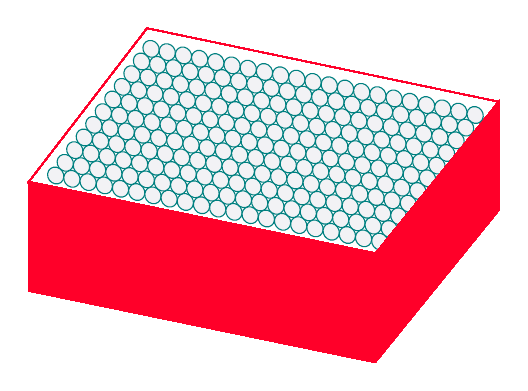
\begin{tikzpicture}[font=\footnotesize, line join=round, line cap=round, >=stealth,scale=.7]
			\definecolor{anti-flashwhite}{rgb}{0.95, 0.95, 0.96}
			\definecolor{ruddy}{rgb}{1.0, 0.0, 0.16}
			\def\r{0.15}
			\foreach \j in {0,...,10}{
				\foreach \i in{0,...,20}{
					\fill[xslant=0.1,yslant=-0.2,anti-flashwhite,draw=teal](2*\i*\r,0)++(60:2*\j*\r)circle(\r);
					
					\draw[xslant=0.77,yslant=-0.18,ruddy](-.4,-.2)rectangle(7,2.6);
					\fill[ruddy](-.5,-.1)--(-.5,-2.1)--(5.8,-3.4)--(5.8,-1.4)--cycle
					(5.8,-3.4)--(5.8,-1.4)--(8.05,1.37)--(8.05,-.63)--cycle;
			}}
		\end{tikzpicture}	
	}
	\loigiai{
		\immini{
			Hình biểu diễn của hộp phấn có thể vẽ như hình bên.
		}{
			\begin{tikzpicture}[line cap=round,line join=round,font=\footnotesize,>=stealth,scale=.8]
				\path
				(0,0) coordinate (A)
				(-1.5,-1.5) coordinate (B)
				(5,0) coordinate (D)
				($(B)+(D)-(A)$)  coordinate (C)
				;
				\coordinate (A') at	($(A)+(0,3)$);
				\coordinate (B') at ($(B)+(A')-(A)$);
				\coordinate (D') at ($(D)+(A')-(A)$);
				\coordinate (C') at ($(B')+(D')-(A')$);
				\draw (A')--(B')--(C')--(D')--cycle (B)--(C)--(D) (B')--(C')--(C) (D)--(D') (B')--(B);
				\draw[dashed] (B)--(A)--(D) (A)--(A');
			\end{tikzpicture}
		}
	}	
\end{vd}
\begin{vd}%[DCHT Toán 11 - KNTT - Võ Trần Khánh Mai]%[1K7BM-6]
	\immini{Hình bên minh họa người thợ đang kiểm tra độ phẳng của mặt sàn nhà. Hãy cho biết người thợ kiểm tra độ phẳng của mặt sàn nhà bằng cách nào?}
	{\includegraphics[scale=0.25]{HINHVE/1}}
	\loigiai{
		Người thợ đặt thước dẹt dài lên mặt sàn nhà ở các vị trí khác nhau. Nếu thước đó luôn áp sát mặt sàn (không bị cập kênh) thì mặt sàn là phẳng.
	}	
\end{vd}
\begin{vd}%[DCHT Toán 11 - KNTT - Võ Trần Khánh Mai]%[1K7BM-6]
	\immini{
		Giải thích tại sao:
		\begin{listEX}
			\item Chân máy ảnh có thể đặt ở hầu hết các loại địa hình mà vẫn đứng vững.
			\item Bàn, ghế bốn chân thường hay bị cập kênh.
	\end{listEX}}
	{
		\includegraphics[scale=0.3]{HINHVE/2}
	}
	\loigiai{
		\begin{listEX}
			\item Giá đỡ ba chân của máy ảnh khi đặt trên mặt đất không bị cập kênh vì theo tính chất \lq\lq Có một và chỉ một mặt phẳng đi qua ba điểm không thẳng hàng cho trước\rq\rq.
			\item Bàn, ghế bốn chân thường hay bị cập kênh vì theo tính chất \lq\lq Tồn tại bốn điểm không cùng nằm trên một mặt phẳng\rq\rq.
		\end{listEX}
	}
\end{vd}
\begin{vd}%[DCHT Toán 11 - KNTT - Võ Trần Khánh Mai]%[1K7BM-6]
	\immini{	Khi trát tường, dụng cụ không thể thiếu của người thợ là thước dẹt dài (hình bên). Công dụng của thước dẹt này là gì? Giải thích.}
	{
		\includegraphics[scale=0.25]{HINHVE/3}
	}
	\loigiai{
		Công dụng của thước dẹt là cán phẳng vữa trên bề mặt tường.\\
		Khi trát tường, người thợ dùng thước dẹt dài di chuyển (cán) trên bề mặt tường làm cho mặt tường phẳng (trùng với mặt phẳng thước). 
	}	
\end{vd}

\subsubsection{Bài tập rèn luyện}
\begin{ex}%[DCHT Toán 11 - KNTT - Võ Trần Khánh Mai]%[1K7BM-6]
	\immini{	Hình bên là hình ảnh của chặn giấy bằng gỗ có bốn mặt phân biệt là các tam giác. Vẽ hình biểu diễn của chặn giấy bằng gỗ đó.}{
		\definecolor{tumbleweed}{rgb}{0.87, 0.67, 0.53}%màu cát
		\begin{tikzpicture}[scale=.7, font=\footnotesize, line join=round, line cap=round, >=stealth]
			\def\bd{5} % cạnh BD
			\def\bc{2} % cạnh BC
			\def\gocB{-30} % góc B của đáy
			\coordinate (B) at (0,0);
			\coordinate (C) at (\gocB:\bc);
			\coordinate (D) at (\bd,0);
			\coordinate (A) at (70:4);
			\fill[tumbleweed] (A)--(B)--(C)--(D)--cycle;
			\draw (A)--(B)--(C)--(D)--cycle (A)--(C);
		\end{tikzpicture}
	}
	\loigiai{
		\immini{
			Hình biểu diễn của chặn giấy bằng gỗ như hình bên.
		}
		{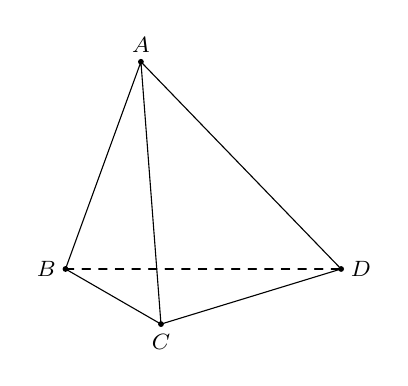
\begin{tikzpicture}[scale=.7, font=\footnotesize, line join=round, line cap=round, >=stealth]
				\def\bd{5} % cạnh BD
				\def\bc{2} % cạnh BC
				\def\gocB{-30} % góc B của đáy
				\coordinate[label=left:$B$] (B) at (0,0);
				\coordinate[label=below:$C$] (C) at (\gocB:\bc);
				\coordinate[label=right:$D$] (D) at (\bd,0);
				\coordinate [label=above:$A$](A) at (70:4);
				\draw (A)--(B)--(C)--(D)--cycle (A)--(C);
				\draw[dashed] (B)--(D);
				
				\foreach \i in {A,B,C,D} \fill[black] (\i) circle (1.5pt);
		\end{tikzpicture}}
	}	
\end{ex}
\begin{ex}%[DCHT Toán 11 - KNTT - Võ Trần Khánh Mai]%[1K7BM-6]
	\immini{
		Thước laser phát ra tia laser, khi tia này quay sẽ tạo ra mặt phẳng ánh sáng. Giải thích tại sao các thước kẻ laser lại giúp người thợ xây dựng kẻ được đường thẳng trên tường hoặc sàn nhà.
	}{\vspace{-0.5cm}
		\includegraphics[scale=0.8]{HINHVE/4}
	}
	\loigiai{
		Thước laser phát ra tia laser; khi quay, các tia laser chung gốc tạo thành một mặt phẳng ánh sáng. \\
		Khi cắt mặt phẳng ánh sáng này bởi mặt tường hoặc sàn nhà thì phần thu được trên tường hoặc sàn là giao tuyến của mặt phẳng ánh sáng và mặt tường hay sàn nhà. Đó là giao tuyến của hai mặt phẳng nên là một đường thẳng.
	}
\end{ex}
\begin{ex}%[DCHT Toán 11 - KNTT - Võ Trần Khánh Mai]%[1K7BM-6]
	\immini{ Chiếc xà ngang đặt tựa lên hai điểm $A$, $B$ của trụ nhảy thể hiện hình ảnh của một đường thẳng đi qua hai điểm đó. Có thể tìm được một đường thẳng khác cũng đi qua hai điểm $A$, $B$ hay không?}{			\includegraphics[width=0.5\linewidth]{HINHVE/5}}
	\loigiai{Không thể tìm được một đường thẳng khác.}	
\end{ex}
\begin{ex}%[DCHT Toán 11 - KNTT - Võ Trần Khánh Mai]%[1K7BM-6]
	Trong Hình $4.4$ là một khối rubik có bốn đỉnh và bốn mặt, mỗi mặt là một tam giác.
	\immini{
		\begin{enumerate}
			\item  Đặt khối rubik sao cho ba đỉnh của mặt màu đỏ đều nằm trên mặt bàn. Khi đó, mặt màu đỏ của khối rubik có nằm trên mặt bàn hay không?
			\item  Có thể đặt khối rubik sao cho bốn đinh của nó đều nằm trên mặt bàn hay không?
	\end{enumerate}}{
		\includegraphics[width=0.5\linewidth]{HINHVE/6}
	}
	\loigiai{\begin{enumerate}
			\item  Mặt màu đỏ của khối rubik nằm trên mặt bàn.
			\item  Không thể đặt khối rubik sao cho bốn đỉnh của nó đều nằm trên mặt bàn.
	\end{enumerate}}
\end{ex}
\begin{ex}%[DCHT Toán 11 - KNTT - Võ Trần Khánh Mai]%[1K7BM-6]
	\immini{ Tại các nhà hàng, khách sạn, nhân viên phục vụ bàn thường xuyên phải bưng bê nhiều khay, đĩa đồ ăn khác nhau. Một trong những nguyên tắc nhân viên cần nhớ là khay phải được bưng bằng ít nhất 3 ngón tay. Hãy giải thích tại sao.}{
		\includegraphics[width=0.5\linewidth]{HINHVE/7}
	}
	\loigiai{Ba đầu ngón tay của nhân viên chính là ba điểm không thẳng hàng. Qua ba điểm không thẳng hàng có duy nhất một mặt phẳng nên khi đó đĩa thức ăn luôn được nằm trên một mặt phẳng xác định. Điều này giữ cho đĩa thức ăn được cân bằng.}
\end{ex}
\begin{ex}%[DCHT Toán 11 - KNTT - Võ Trần Khánh Mai]%[1K7BM-6]
	\immini{ 
		Bàn cắt giấy là một dụng cụ được sử dụng thường xuyên ở các cửa hàng photo-copy. Bàn cắt giấy gồm hai phần chính: phần bàn hình chữ nhật có chia kích thước giấy và phần dao cắt có một đầu được cố định vào bàn. Hãy giải thích tại sao khi sử dụng bàn cắt giấy thì các đường cắt luôn là đường thẳng.}{\includegraphics[width=0.5\linewidth]{HINHVE/8}}
	\loigiai{Đường cắt tạo ra từ dao cắt và bàn cắt hình chữ nhật chính là giao tuyến của hai mặt phẳng: mặt phẳng xác định từ lưỡi của dao cắt và mặt phẳng xác định từ bàn cắt hình chữ nhật nên đường cắt luôn là đường thẳng.
	}
\end{ex}

\Closesolutionfile{ans}